\documentclass{article}

\usepackage{graphicx}
\usepackage{tikz}
\usepackage{tikzsymbols}
\usetikzlibrary{calc,patterns,shapes.geometric}
\pagestyle{empty}
\usepackage[margin=0pt]{geometry}
\geometry{papersize={14in,12in}}

\def\centerarc[#1](#2)(#3:#4:#5){\draw[#1] ($(#2)+({#5*cos(#3)},{#5*sin(#3)})$) arc (#3:#4:#5);}

\begin{document}
	\begin{figure}
		\centering
		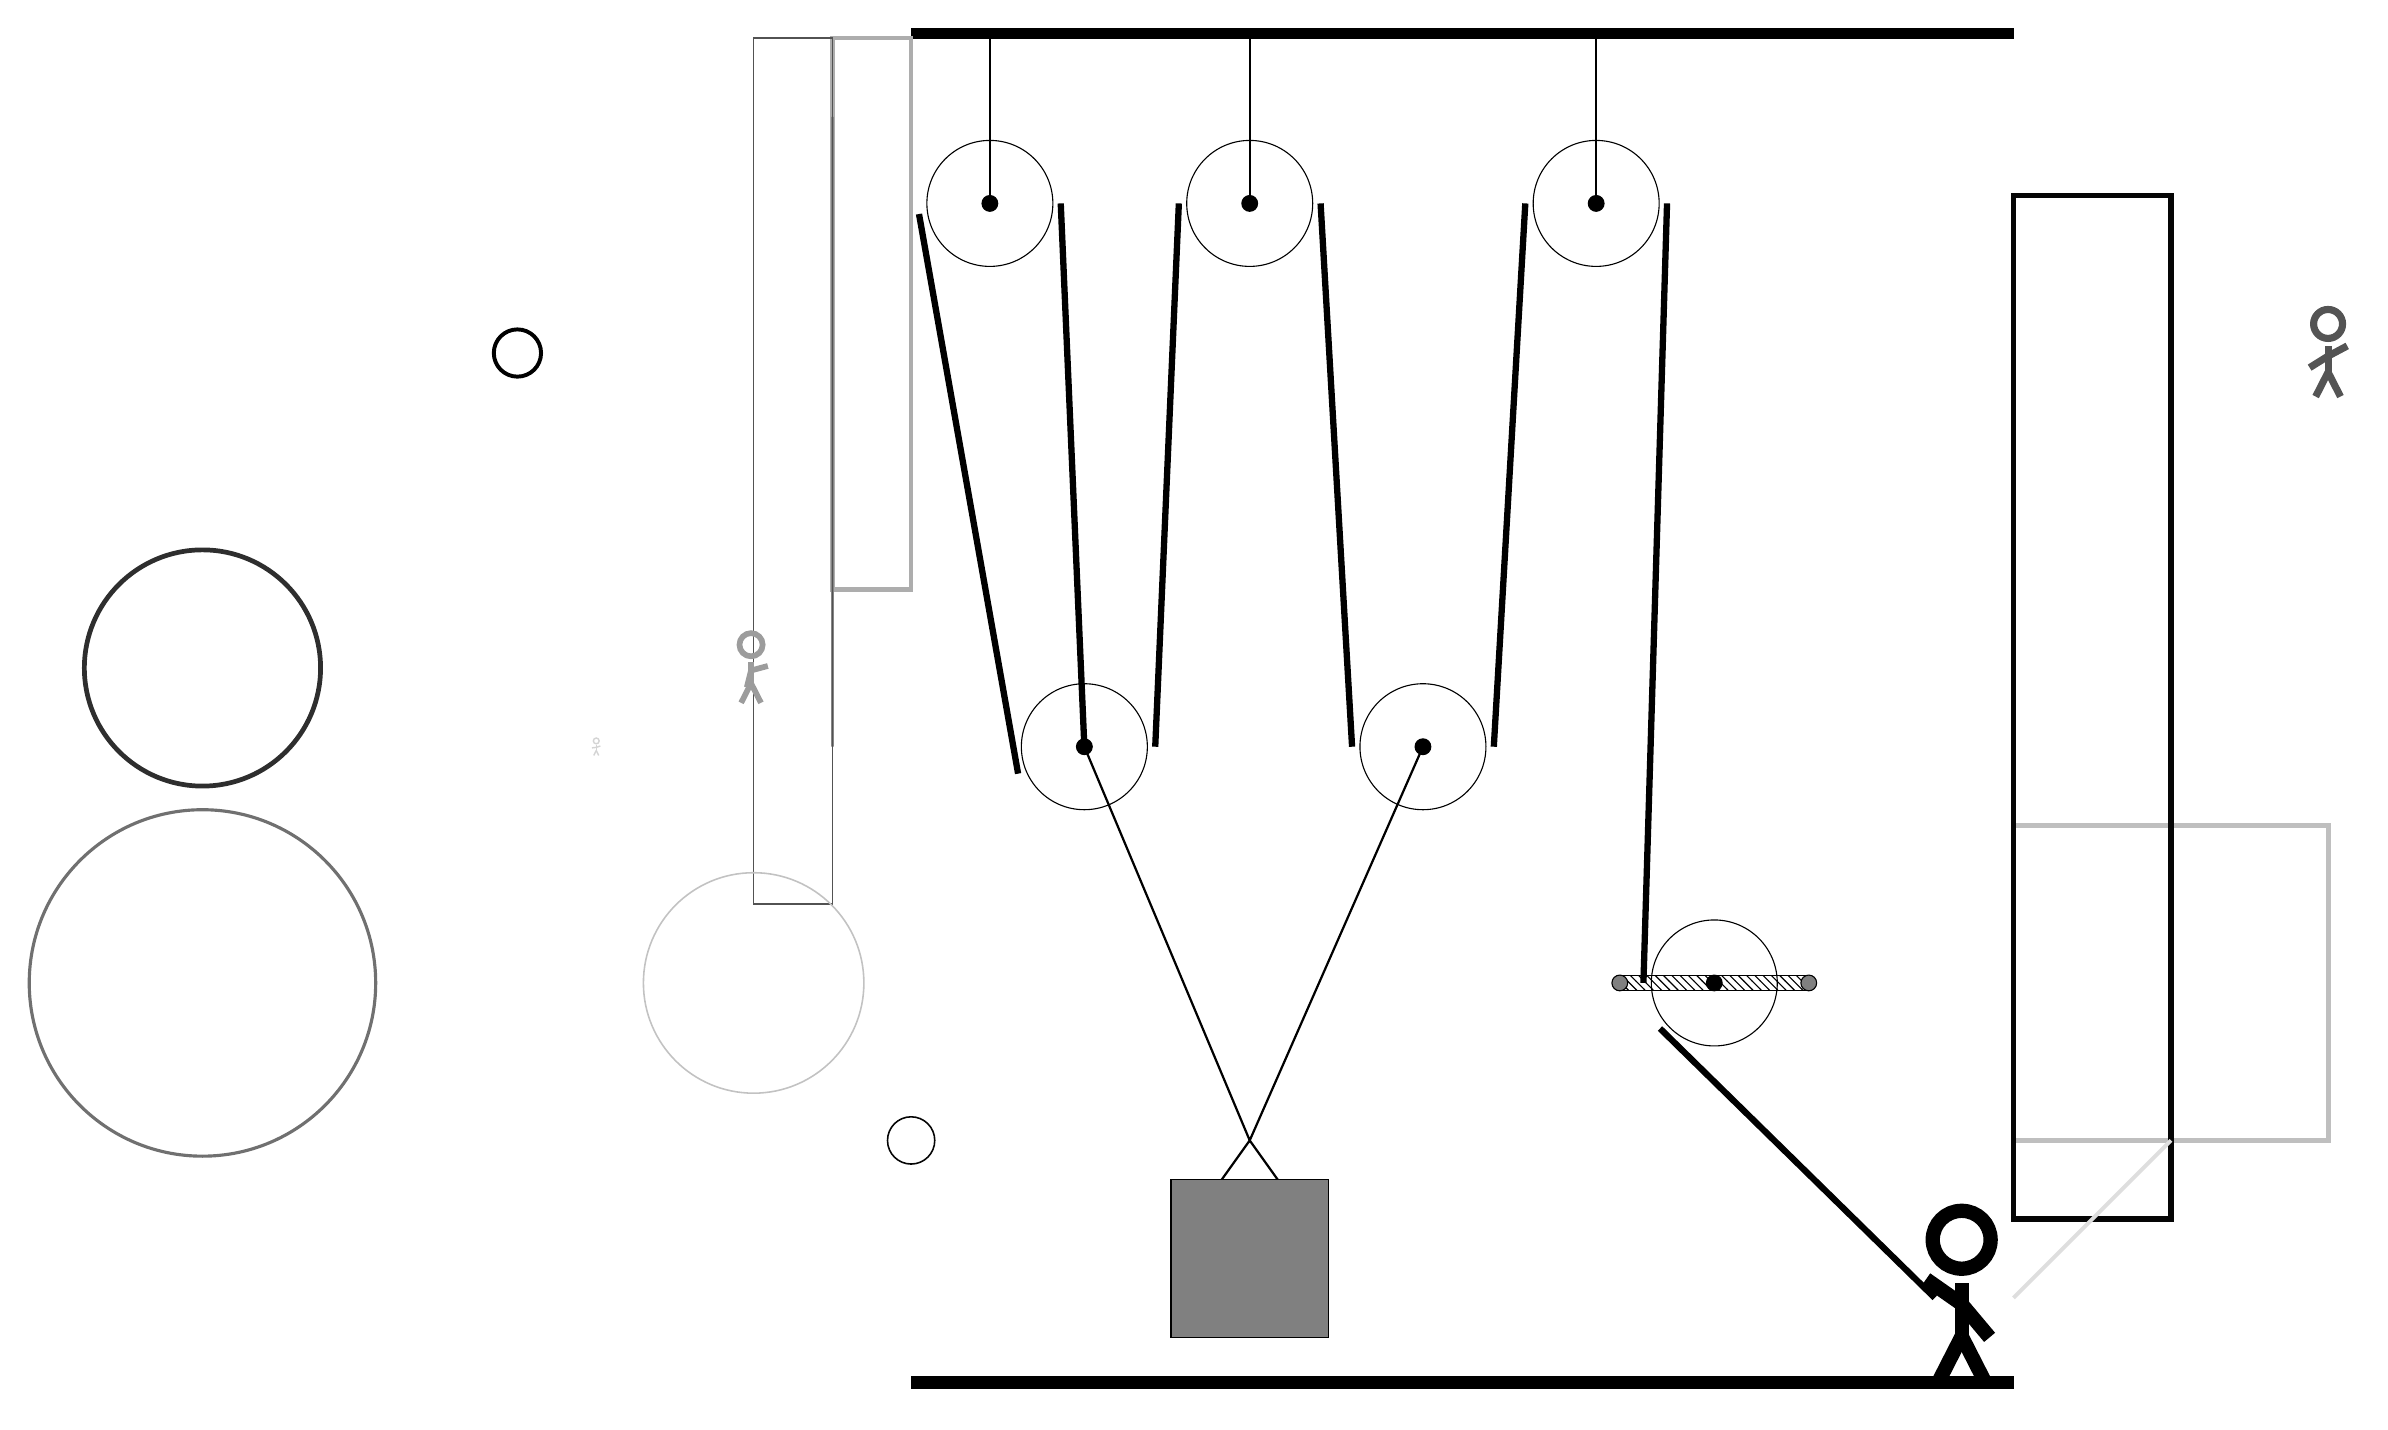
\begin{tikzpicture}
			%%%%% START %%%%%
			
			\draw[fill=black] (-2, 14) rectangle (12, 14.125);
			
			\draw (-1, 11.9) circle (0.8);
			\draw[fill=black] (-1, 11.9) circle (0.1);
			\draw[thick] (-1, 11.9) -- (-1, 14);
			
			\draw (2.3, 11.9) circle (0.8);
			\draw[fill=black] (2.3, 11.9) circle (0.1);
			\draw[thick] (2.3, 11.9) -- (2.3, 14);
			
			\draw (6.7, 11.9) circle (0.8);
			\draw[fill=black] (6.7, 11.9) circle (0.1);
			\draw[thick] (6.7, 11.9) -- (6.7, 14);
			
			\draw (0.2, 5) circle (0.8);
			\draw[fill=black] (0.2, 5) circle (0.1);
			
			\draw (4.5, 5) circle (0.8);
			\draw[fill=black] (4.5, 5) circle (0.1);
			
			\draw (8.2, 2) circle (0.8);
			\draw[fill=black] (8.2, 2) circle (0.1);
			\draw[pattern=north west lines, pattern color=black] (7.0, 2.1) rectangle (9.4, 1.9);
			\draw[fill=black!50] (7.0, 2) circle (0.1);
			\draw[fill=black!50] (9.4, 2) circle (0.1);
			
			\draw[line width=0.6mm, color=black!32] (-3, 7) rectangle (-2, 14);
			
			\draw [line width=0.2mm, color=black!98](-2, 0) circle (0.3);
			\draw [line width=0.5mm, color=black!100](-7, 10) circle (0.3);
			\draw[line width=0.3mm, color=black!48] (-3, 5) rectangle (-3, 13);
			\draw[line width=0.7mm, color=black!25] (12, 4) rectangle (16, 0);
			\draw[line width=0.2mm, color=black!68] (-3, 14) rectangle (-4, 3);
			\draw [line width=0.6mm, color=black!82](-11, 6) circle (1.5);
			
			\node[line width=0.2mm, color=black!17] at (-6, 5) {\Strichmaxerl[1][7][18]};
			\draw[line width=0.7mm, color=black!98] (14, -1) rectangle (12, 12);
			
			\draw [line width=0.4mm, color=black!56](-11, 2) circle (2.2);
			\draw [line width=0.2mm, color=black!24](-4, 2) circle (1.4);
			\draw[line width=0.5mm, color=black!13](14, 0) -- (12, -2);
			\node[line width=0.3mm, color=black!67] at (16, 10) {\Strichmaxerl[5][32][28]};
			
			\node[line width=0.5mm, color=black!39] at (-4, 6) {\Strichmaxerl[4][76][15]};
			
			\draw[thick] (0.2, 5) -- (2.3, 0)  -- (4.5, 5);
			\draw[thick]  (1.8, -0.7) -- (2.3, 0) -- (2.8, -0.7);
			\draw[fill=black!50] (1.3, -0.5) rectangle (3.3, -2.5);
			
			\draw[line width=0.8mm] (0.2, 5) -- (-0.1, 11.9);
			\centerarc[line width=0.8mm](-1, 11.9)(0:200:0.9);
			\draw[line width=0.8mm] (-1.9, 11.765) -- (-0.6415, 4.658);
			\centerarc[line width=0.8mm](0.2, 5)(200:360:0.9);
			\draw[line width=0.8mm](1.1, 5) -- (1.4, 11.9);
			\centerarc[line width=0.8mm](2.3, 11.9)(0:180:0.9);
			\draw[line width=0.8mm] (3.2, 11.9) -- (3.6, 5);
			\centerarc[line width=0.8mm](4.5, 5)(180:360:0.9);
			\draw[line width=0.8mm] (5.4, 5) -- (5.8, 11.9);
			\centerarc[line width=0.8mm](6.7, 11.9)(0:180:0.9);
			\draw[line width=0.8mm](7.6, 11.9) --  (7.3, 2);
			\centerarc[line width=0.8mm](8.2, 2)(180:220:0.9);
			\draw[line width=0.8mm](7.5106, 1.4215) -- (11, -2);
			
			\node at (11.3, -2) {\Strichmaxerl[10][-35][-50]};
			
			\draw[fill=black] (-2, -3) rectangle (12, -3.15);
			
			%%%%% END %%%%%
		\end{tikzpicture}
	\end{figure}	
\end{document}